\documentclass[paper=a4, fontsize=11pt]{scrartcl} % A4 paper and 11pt font size
\usepackage[T1]{fontenc}  % proper encoding for output file
\usepackage[utf8]{inputenc}  % except UTF-8 character in source
\usepackage[english]{babel}  % set document language
\usepackage{amsmath,amsfonts,amsthm}  % math type setting
\usepackage{mhchem}  % chemical expressions
\usepackage{graphicx}  % inclue graphics
\usepackage{url}
\usepackage{caption}
\usepackage{subcaption}
\setlength\parindent{0pt} % Removes all indentation from paragraphs


\title{Exercise 1: Calculation of Absorption Coefficients}
\author{Sample Solution}
\date{Effective: 19.10.2016}

%%%%%%%%%%%%%%%%%%%%%%%%%%%%%%%%%%%%%%%%%%%%%%%%%%%%%%%%%%%%%%%%%%%%%%%%%%%%%%%
\begin{document}

\maketitle

\section{Pressure dependency of the abs cross section}
Choose an individual line and perform calculations over a restricted frequency
range for four different pressures (1\,hPa, 10\,hPa, 100\,hPa, 1000\,hPa).
Keep the temperature and constituent mixing ratio constant.

% figures abs cross sections
\begin{figure}[ht]
    \centering
    \begin{subfigure}[t]{0.45\textwidth}
        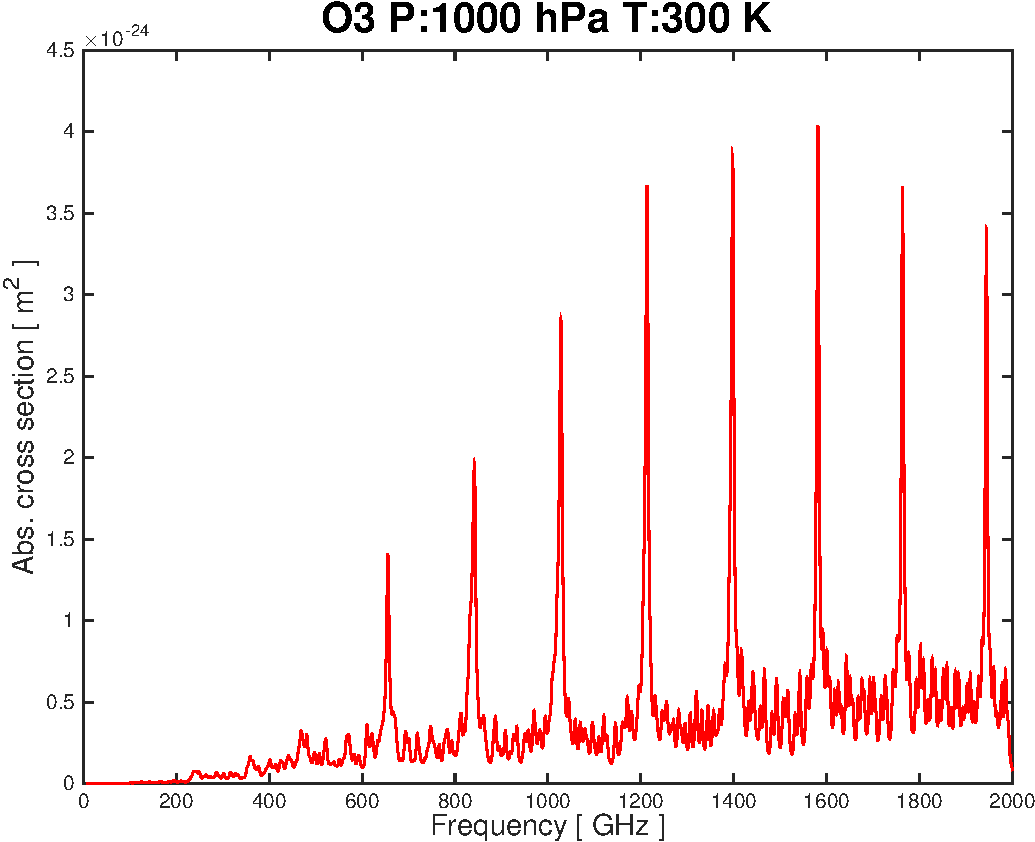
\includegraphics[width=\textwidth]{plots/plot_xsec_O3_1000hPa_300K.pdf}
        \caption{1000\,hPa}
    \end{subfigure}
    \begin{subfigure}[t]{0.45\textwidth}
        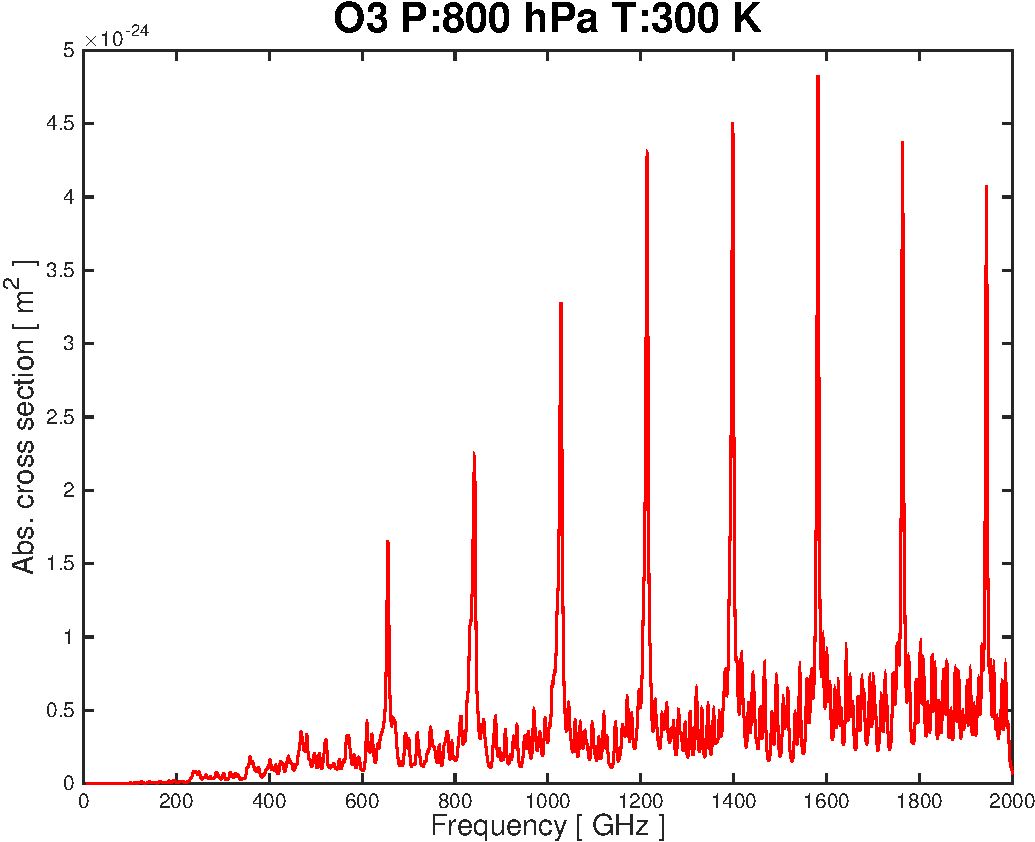
\includegraphics[width=\textwidth]{plots/plot_xsec_O3_800hPa_300K.pdf}
        \caption{800\,hPa}
    \end{subfigure}
    \begin{subfigure}[b]{0.45\textwidth}
        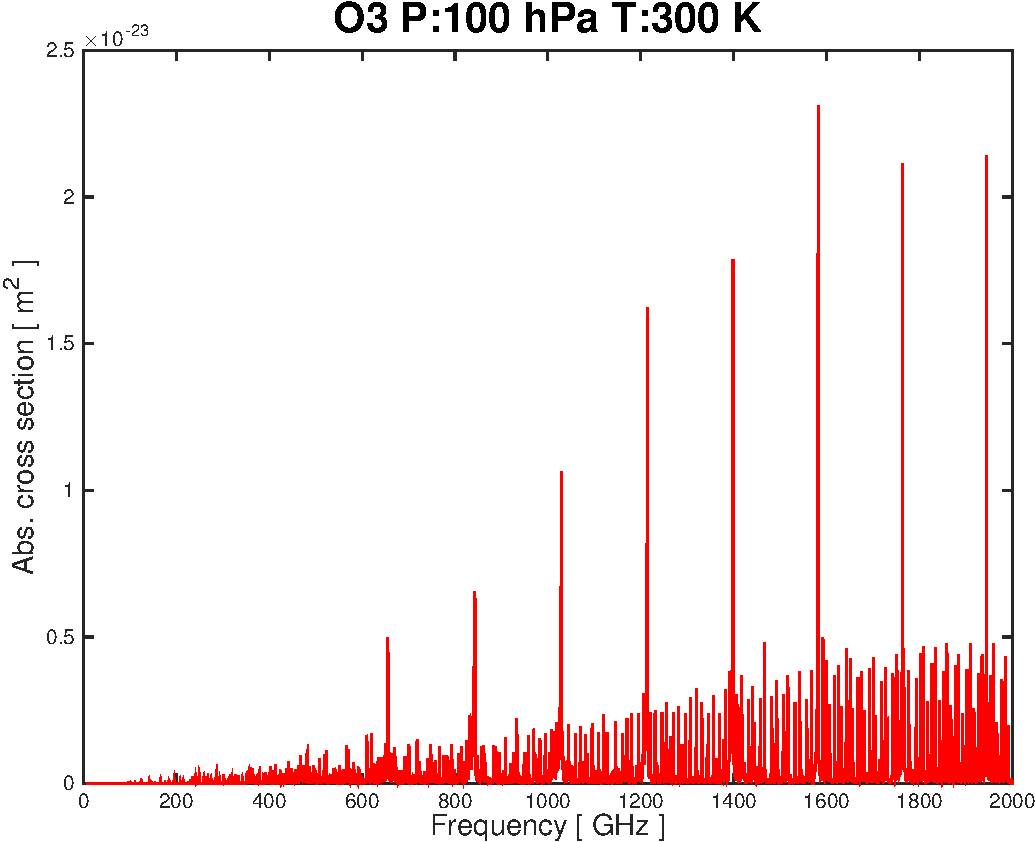
\includegraphics[width=\textwidth]{plots/plot_xsec_O3_100hPa_300K.pdf}
        \caption{100\,hPa}
    \end{subfigure}
    \begin{subfigure}[b]{0.45\textwidth}
        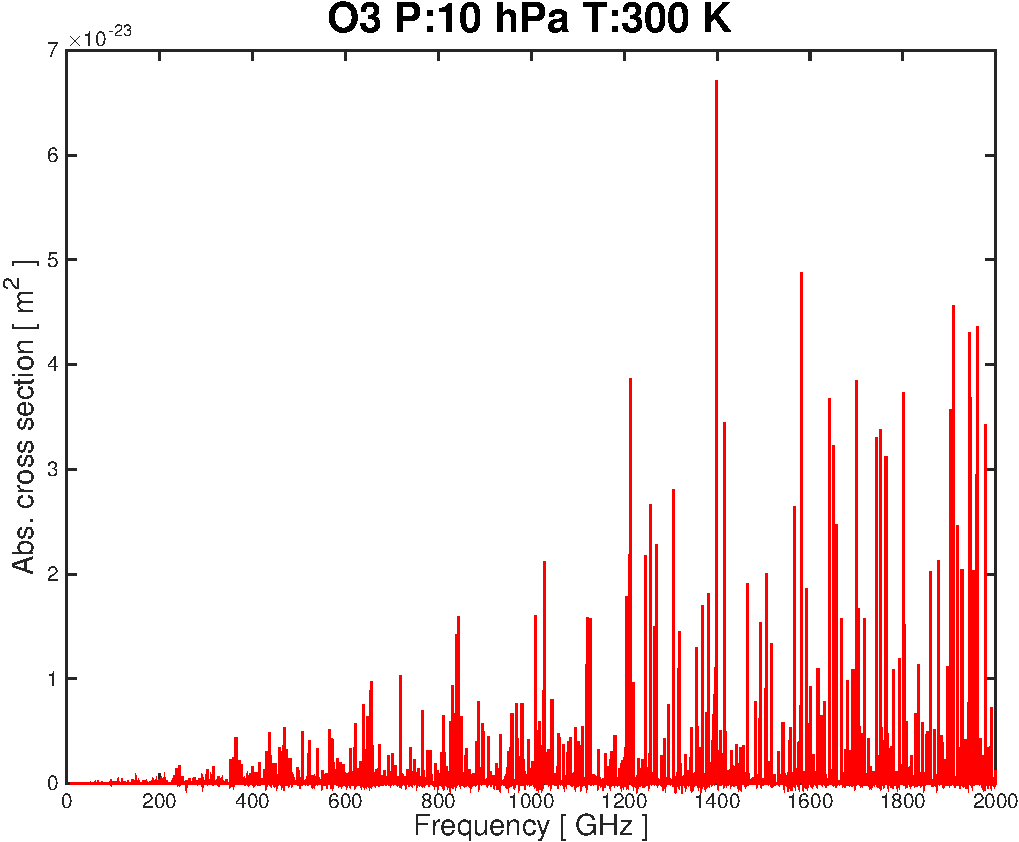
\includegraphics[width=\textwidth]{plots/plot_xsec_O3_10hPa_300K.pdf}
        \caption{10\,hPa}
    \end{subfigure}

    \caption{absorption cross sections for O3 at two different pressure levels.}
    \label{fig:abs_pressure}
\end{figure}

\begin{itemize}
    \item How does the shape of the spectral lines change?
    \begin{itemize}
        \item The lines get wider with increasing pressure. This phenomena is called pressure broadening.
    \end{itemize}
    \item How does the absorption coefficient in the line center change, if pressure is changed?
    \begin{itemize}
        \item The absorption coefficient in the line center decreases with higher pressure.
    \end{itemize}
\end{itemize}
\end{document}

\end{document}
